\subsection[Схема Шамира]{Схема разделения секрета Шамира}\index{схема разделения секрета!Шамира|(}\index{схема разделения секрета!интерполяционных полиномов Лагранжа|(}
\selectlanguage{russian}

Схема разделения секрета Шамира (\langen{Adi Shamir},~\cite{Shamir:1979}), также называемая схемой интерполяционных полиномов Лагранжа, основывается на том, что для восстановления всех коэффициентов полинома $P(x) = a_{K-1}x^{K-1} + \dots + a_1 x + a_0$ степени $K-1$ требуется $K$ координат различных точек, принадлежащих кривой $y=P(x)$. Все операции проводятся в конечном поле $GF(p)$.

\begin{figure}[thb]
	\centering
	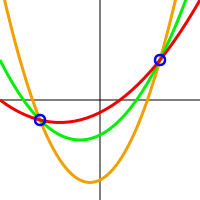
\includegraphics[width=0.5\textwidth]{pic/shamir}
  \caption{Через две точки можно провести неограниченное число графиков, заданных полиномами степени 2. Для выбора единственного из них нужна третья точка. Данные графики приведены только для иллюстрации идеи: в схеме Шамира используется конечное поле, полиномы над которым сложно представить на графике.}
  \label{fig:shamir}
\end{figure}

Для разделения секрета $M$ между $N$ сторонами таким образом, чтобы любые $K$ сторон могли восстановить секрет, доверенный центр выполняет следующие операции:
\begin{itemize}
	\item выбирает несекретное большое простое число $p$ ($p > M$);
	\item в качестве свободного члена секретного многочлена полагает разделяемый секрет $a_0 = M$;
	\item выбирает остальные секретные коэффициенты многочлена $a_1, \dots, a_{k-1}$, меньшие, чем $p$;
	\item выбирает $N$ различных $x$, таких, что $0 < x_i < p$;
	\item для каждого выбранного $x_i$ вычисляет соответствующий $y_i$, подставляя значения в формулу многочлена
		\[ y_i = P( x_i ) = a_{K-1}x_i^{K-1} + \dots + a_1 x_i + a_0 \mod p ;\]
	\item раздаёт каждой стороне по следу вида $(x_i, y_i)$ и общему модулю $p$.
\end{itemize}

Если стороны могут собраться вместе и получить не менее чем $K$ различных следов, то, составив и решив систему уравнений с $K$ неизвестными, они смогут получить все коэффициенты $a_0, a_1, \dots, a_{k-1}$ секретного многочлена:
\[ \left\{ \begin{array}{l}
    y_1 = a_{K-1}x_1^{K-1} + \dots + a_1 x_1 + a_0 \mod p, \\
    \dots, \\
    y_k = a_{K-1}x_k^{K-1} + \dots + a_1 x_k + a_0 \mod p. \\
\end{array} \right. \]

Если собрано меньшее количество следов, то их будет недостаточно для решения системы уравнений.

Существует также способ вычисления коэффициентов многочлена, основанный на методе интерполяционных полиномов Лагранжа (откуда и берётся второе название метода разделения секрета). Идея способа состоит в вычислении набора специальных полиномов $l_i \left( x \right)$, которые принимают значение $1$ в точке $x_i$, а во всех остальных точках-следах их значение равно нулю:
\[ \begin{cases}
	l_i \left( x_j \right) = 1, &x_j = x_i, \\
	l_i \left( x_j \right) = 0, &x_j \ne x_i. \\
\end{cases} \]

Далее эти многочлены умножаются на значения $y_i$ и в сумме дают исходный многочлен:
\[\begin{array}{llll}
  l_i \left( x \right) &=& \prod\limits_{j \ne i} {\frac{{x - x_j }}{{x_i  - x_j }}} &\mod p, \\
  F\left( x \right) &=& \sum\limits_i {l_i \left( x \right)y_i } &\mod p. \\
\end{array}\]

Строго говоря, для восстановления самого секрета, которым является свободный член многочлена, не обязательно восстанавливать весь многочлен, а можно использовать упрощённую формулу для восстановления только свободного члена $a_0 = M$:
    \[ M = \sum\limits_{i=0}^{k-1} y_i \prod\limits_{j=0, j \neq i}^{k-1} \frac{x_j}{x_j - x_i}. \]

\example
Приведём схему Шамира в поле $\GF{p}$. Для разделения секрета $M$ в $(3,n)$-пороговой схеме используется многочлен степени $3-1=2$.
    \[ f(x) = a x^2 + b x + M \mod p, \]
где $p$ -- простое\index{число!простое} число. Пусть $p=23$. Восстановим секрет $M$ по \emph{теням}
    \[ (1,14), (4,21), (15,6). \]

Последовательно вычисляем
\[\begin{array}{llc}
M	&\displaystyle = \sum\limits_{i=0}^{k-1} y_i \prod\limits_{j=0, j \neq i}^{k-1} \frac{x_j}{x_j - x_i} & \mod p = \\
	\\
	&= 14 \cdot \frac{4}{4-1} \cdot \frac{15}{15-1} + 21 \cdot \frac{1}{1-4} \cdot \frac{15}{15-4} + 6 \cdot \frac{1}{1-15} \cdot \frac{4}{4-15} & \mod 23 = \\
	\\
	&\displaystyle = 14 \cdot \frac{4}{3} \cdot \frac{15}{14} + 21 \cdot \frac{1}{-3} \cdot \frac{15}{11} + 6 \cdot \frac{1}{-14} \cdot \frac{4}{-11} & \mod 23 = \\
	\\
	&\displaystyle = 20 - 7 \cdot 15 \cdot 11^{-1} + 12 \cdot 7^{-1} \cdot 11^{-1} & \mod 23 = \\
	\\
	&= 13 \mod 23.
\end{array}\]

\exampleend

\index{схема разделения секрета!интерполяционных полиномов Лагранжа|)}\index{схема разделения секрета!Шамира|)}
